%  ProgGuide.tex
%  Document created by seblovett on hind.ecs.soton.ac.uk
%  Date created: Thu 27 Mar 2014 10:09:06 GMT
%  <+Last Edited: Wed 30 Apr 2014 08:18:48 BST by seblovett on seblovett-Ubuntu +>

\documentclass[twoside,12pt]{article}

%\usepackage[nodayofweek]{datetime}
\usepackage{ISFormat}
\usepackage{multirow}
\usepackage[colorinlistoftodos]{todonotes}
\usepackage[nodayofweek]{datetime}
\usepackage{listings}
\usepackage{graphicx}
\usepackage{titlesec}
\newcommand{\sectionbreak}{\cleardoublepage}
\usepackage[all]{background}
\usepackage{lipsum}
\usepackage{tikz}
\usetikzlibrary{calc}
\usepackage{changepage}

\graphicspath{{Figures/}}
\author{Team R4\\
Henry Lovett (hl13g10)\\ 
Ashey J. Robinson (ajr2g10)\\
Martin Wearn (mw20g10)\\
Anusha R. Reddy (arr1g13)\\ \\
Course Tutor: Mr B. Iain McNally\\ \\}

\title{ELEC6027 - VLSI Design Project \\ Programmers Guide}

\begin{document}
\maketitle
\thispagestyle{empty}
%  definitions.tex
%  Document created by seblovett on seblovett-Ubuntu
%  Date created: Thu 24 Apr 2014 18:25:35 BST
%  <+Last Edited: Thu 24 Apr 2014 18:40:49 BST by seblovett on seblovett-Ubuntu +>

% This contains macros and definitions used in the report. 

\definecolor{mygreen}{rgb}{0,0.6,0}
\definecolor{mygray}{rgb}{0.5,0.5,0.5}
\definecolor{mymauve}{rgb}{0.58,0,0.82}

%Code Styles
\lstset{basicstyle=\scriptsize\ttfamily,
  backgroundcolor=\color{white},   % choose the background color; you must add \usepackage{color} or \usepackage{xcolor}
  basicstyle=\footnotesize,        % the size of the fonts that are used for the code
  breakatwhitespace=false,         % sets if automatic breaks should only happen at whitespace
  breaklines=true,                 % sets automatic line breaking
  captionpos=t,                    % sets the caption-position to bottom
  commentstyle=\color{mygreen},    % comment style
  deletekeywords={...},            % if you want to delete keywords from the given language
  escapeinside={\%*}{*)},          % if you want to add LaTeX within your code
  extendedchars=true,              % lets you use non-ASCII characters; for 8-bits encodings only, does not work with UTF-8
  frame=single,                    % adds a frame around the code
  keepspaces=true,                 % keeps spaces in text, useful for keeping indentation of code (possibly needs columns=flexible)
  numbers=left,                    % where to put the line-numbers; possible values are (none, left, right)
  numbersep=5pt,                   % how far the line-numbers are from the code
  numberstyle=\tiny\color{mygray}, % the style that is used for the line-numbers
  rulecolor=\color{black},         % if not set, the frame-color may be changed on line-breaks within not-black text (e.g. comments (green here))
  showspaces=false,                % show spaces everywhere adding particular underscores; it overrides 'showstringspaces'
  showstringspaces=false,          % underline spaces within strings only
  showtabs=false,                  % show tabs within strings adding particular underscores
  stepnumber=1,                    % the step between two line-numbers. If it's 1, each line will be numbered
  tabsize=2,                       % sets default tabsize to 2 spaces
  title=\lstname                   % show the filename of files included with \lstinputlisting; also try caption instead of title
}
\lstdefinestyle{C} {
  language=C,
  otherkeywords={uint16_t,uint32_t,uint8_t},
  stringstyle=\color{mymauve},     % string literal style
  keywordstyle=\color{blue}      % keyword style
}
\lstdefinestyle{sverilog} {
  language=Verilog,
  otherkeywords={always\_ff,always\_comb,assert,logic,return,\$random,\#*},            % if you want to add more keywords to the set
  stringstyle=\color{mymauve},     % string literal style
  keywordstyle=\color{blue}      % keyword style
}
\lstdefinestyle{asm} {
  otherkeywords={ADD,ADDI,ADDIB,ADC,ADCI,NEG,SUB,SUBIB,SUC,SUCI,CMP,CMPI,AND,OR,XOR,NOT,NAND,NOR,LSL,LSR,ASR,LDW,STW,LUI,LLI,BR,BNE,BE,BLT,BGE,BWL,RET,JMP,PUSH,POP,RETI,ENAI,DISI,STF,LDF},            % if you want to add more keywords to the set
  keywordstyle=\color{blue},       % keyword style
  language={[x86masm]Assembler}                % the language of the code
}


%import some definitions
\clearpage
\listoftodos
%\todo[inline]{Run a spell check on all files}
%\begin{abstract}
%Abstract
%\end{abstract}
\cleardoublepage
\tableofcontents
\cleardoublepage
%  Introduction.tex
%  Document created by seblovett on seblovett-Ubuntu
%  Date created: Thu 17 Apr 2014 14:53:54 BST
%  <+Last Edited: Sun 11 May 2014 10:39:53 BST by seblovett on seblovett-Ubuntu +>


\chapter{Introduction}

%incomplete{Introduction}
\review{Introduction}

This report documents the design and test of the \textsc{Samurai} processor. 
The processor was designed for the ELEC6027: VLSI design module by Team R4.

The report is broken down into four main sections.
Firstly, the overall design of the architecture and instruction set are discussed. 
The design of the processor, including all datapath modules and the behavioural model for the controller, is then discussed.
This includes state machines and circuit diagrams where applicable. 
Following the design, the testing is documented. 
This includes descriptions of the tests conducted on all designed modules. 
Finally, the report concludes. 


%  Architecture.tex
%  Document created by seblovett on seblovett-Ubuntu
%  Date created: Thu 17 Apr 2014 14:55:41 BST
%  <+Last Edited: Sun 11 May 2014 10:13:31 BST by seblovett on seblovett-Ubuntu +>


\chapter{Architecture}

\incomplete{Architecture}

Design of the datapath architecture.

Refer to the research done and how this influenced the design

The architecture for the processor was initially base upon a MIPS style datapath.
Support was then added to allow the ARM Thumb instruction set (see Chapter~\ref{ch:is}) to be executed on the datapath. \todo[inline, color=green]{MW: `instruction set' makes more sense than `architecture' since the latter is more physical hardware than tasks to be performed}
Extra aspects of the datapath were then added based on the research done. 
The full datapath diagram is seen in Figure~\ref{fig:architecture}.

A Link Register is used to improve the speed when calling leaf functions.
\todo[inline, color=green]{MW: doesnt sound right, use of word `dedicated' would be good}
The original design also included a dedicated Stack Pointer, however this was later removed during the project.
\todo[inline, color=green]{MW: why was it?}
The convention of using Register 7 as the Stack Pointer was instead used. 

The datapath was also modified during the project to allow for interrupt support.
These changes included an input to the Program Counter to jump to a specific location, reading and writing of the status register from and to the system bus, and input of the Program Counter directly from the system bus. 

\inote{HSL: I don't know how in depth we should go here as we talk about everything later on}

\begin{figure}
%%\missingfigure{Architecture diagram}
%\hspace*{-1in}
\vspace*{-1in}
\setlength{\abovecaptionskip}{0pt}
\setlength{\belowcaptionskip}{0pt}
\makebox[\linewidth]{
\centerline{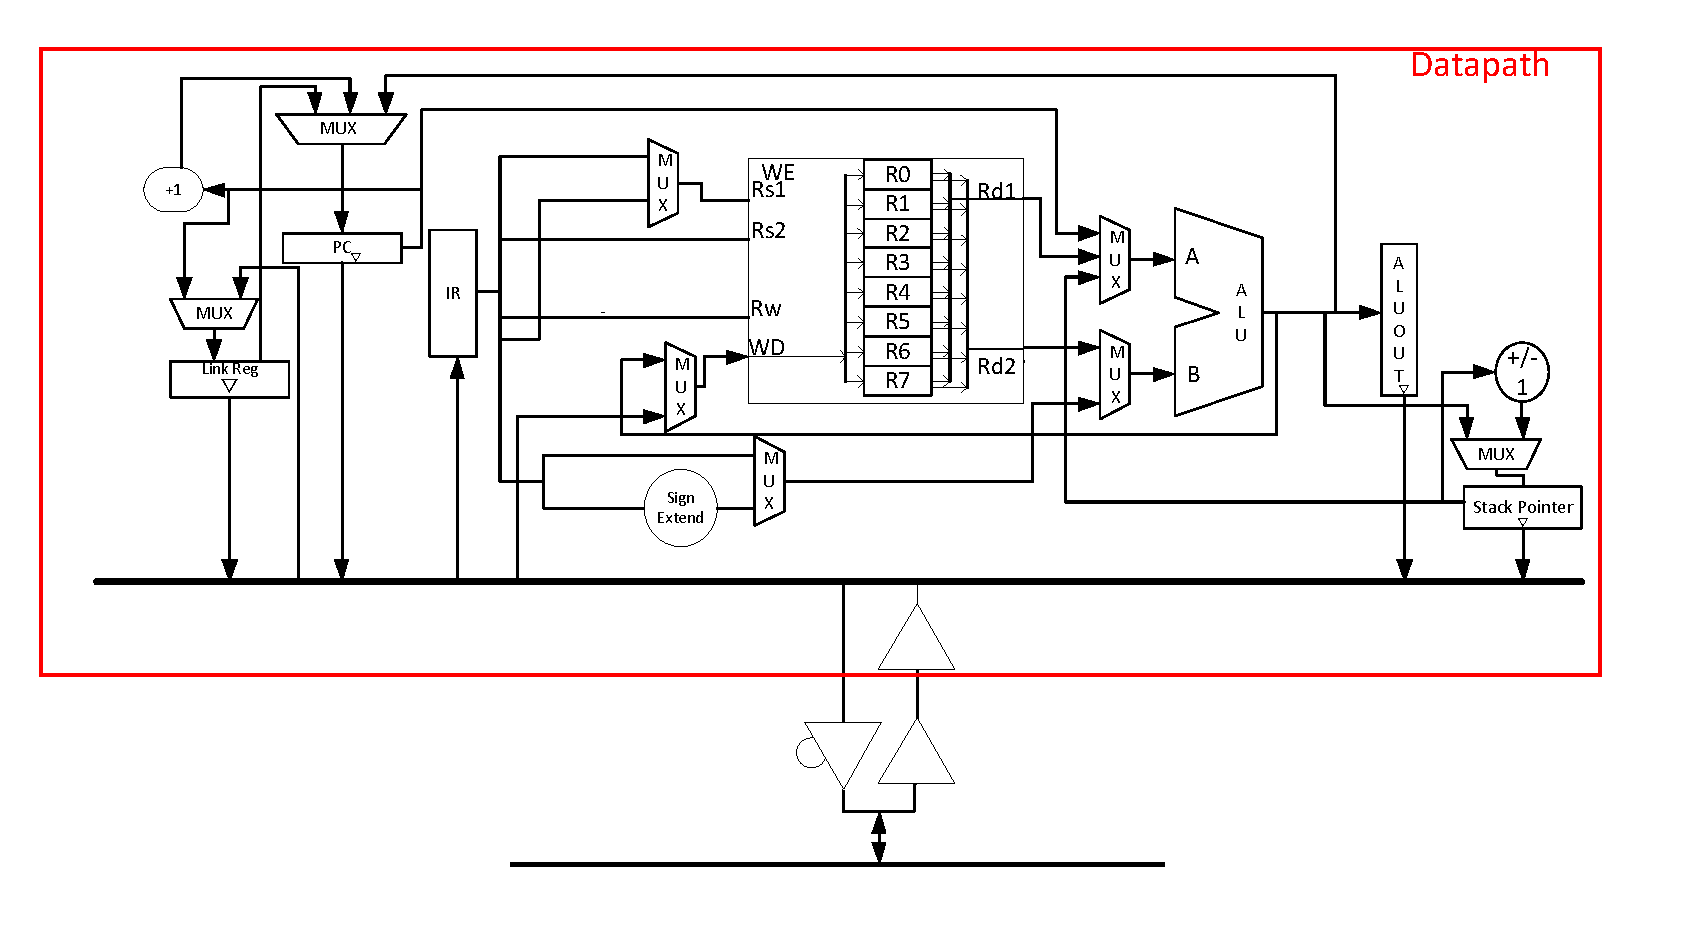
\includegraphics[angle=270,scale=0.9]{../../Design/RandD/idea1.pdf}}
}
\caption{The Architecture diagram of the processor.}
\label{fig:architecture}
\end{figure}
\todo[inline, color=green]{MW: would this need re-angling so bottom edge on outside edge of book?}


%  RegDescription.tex
%  Document created by seblovett on hind.ecs.soton.ac.uk
%  Date created: Thu 27 Mar 2014 10:12:06 GMT
%  <+Last Edited: Thu 27 Mar 2014 10:12:20 GMT by hl13g10 on hind.ecs.soton.ac.uk +>

\section{Register Description}
Lorem Ipsum\dots


%  InstructionSet.tex
%  Date created: Thu 27 Mar 2014
%  <+Last edited: Sat 05 apr 2014 by mw20g10

\newpage
\section{Instruction Set}

The complete instruction set architecture includes a number of instructions for performing calculations on data, memory access, transfer of control\todo{HSL - this doesn't sound right. Maybe "transfer of program flow". Not sure on the use of the word "control" but i know it is the technical term} within a program and interrupt handling.\todo{HSL - this is a bit too short. Surely there is more to say about it?} 

\vspace{\baselineskip}
\noindent All instructions implemented by this architecture fall into one of 6 groups, categorized as follows:
\begin{itemize}
	\item Data Manipulation - Arithmetic, Logical, Shifting
	\item Byte Immediate - Arithmetic, Byte Load
	\item Data Transfer - Memory Access
	\item Control Transfer - (Un)conditional Branching
	\item Stack Operations - Push, Pop
	\item Interrupts - Enabling, Status Storage, Returning
\end{itemize}

\vspace{\baselineskip}
\noindent There is only one addressing mode associated with each instruction, generally following these groupings:
\begin{itemize}
	\item Data Manipulation - Register-Register, Register-Immediate
	\item Byte Immediate - Register-Immediate
	\item Data Transfer - Base Plus Offset
	\item Control Transfer - PC Relative, Register-Indirect, Base Plus Offset
	\item Stack Operations - Register-Indirect Preincrement/Postdecrement
	\item Interrupts - Register-Indirect Preincrement/Postdecrement
\end{itemize}
\vspace{\baselineskip}

\newpage

\subsection{General Instruction Formatting}
\todo[inline]{HSL - I remember Iain saying something about the instruction formats being called A1 / A2. I don't see a problem personally as I can't remember exactly what he said!}
%\newcolumntype{B}{>{\begin{varwidth}{0.2cm}} c <{\end{varwidth}}}
\newcolumntype{B}{c}
\begin{table}[h]
\centering
\footnotesize
\setlength{\tabcolsep}{2.5pt}
\makebox[\linewidth]{
\begin{tabular}{|r|l|l||BBBBBBBBBBBBBBBc|}
	 \multicolumn{1}{r}{} & \multicolumn{1}{l}{\bf Instruction Type} & \multicolumn{1}{l}{\bf Sub-Type} & 15 & 14 & 13 & 12 & 11 & 10 & 9 & 8 & 7 & 6 & 5 & 4 & 3 & 2 & 1 & \multicolumn{1}{B}{0} \\
	\hline
	A1 & \multirow{2}{*}{\bf Data Manipulation} & {\bf Register} & \multicolumn{5}{B|}{\multirow{2}{*}{Opcode}} & \multicolumn{3}{B|}{Rd} & \multicolumn{3}{B|}{Ra} & \multicolumn{3}{B|}{Rb} & X & X \\
	\cline{1-1} \cline{3-3} \cline{9-19}
	A2 &  & {\bf Immediate} & \multicolumn{5}{B|}{} & \multicolumn{3}{B|}{Rd} & \multicolumn{3}{B|}{Ra} & \multicolumn{5}{B|}{imm4/5} \\
	\hline
	B & \multicolumn{2}{l||}{\bf Byte Immediate} & \multicolumn{5}{B|}{Opcode} & \multicolumn{3}{B|}{Rd} & \multicolumn{8}{B|}{imm8} \\
	\hline
	C & \multicolumn{2}{l||}{\bf Data Transfer} & 0 & \multicolumn{1}{|B|}{LS} & 0 & 0 & \multicolumn{1}{B|}{0} & \multicolumn{3}{B|}{Rd}  &\multicolumn{3}{B|}{Ra} & \multicolumn{5}{B|}{imm5} \\
	\hline
	D1 & \multirow{2}{*}{\bf Control Transfer} & {\bf Others} & \multirow{2}{*}{1} & \multirow{2}{*}{1} & \multirow{2}{*}{1} & \multirow{2}{*}{1} & \multicolumn{1}{B|}{\multirow{2}{*}{0}} & \multicolumn{3}{B|}{\multirow{2}{*}{Cond.}}  & \multicolumn{8}{B|}{imm8} \\
	\cline{1-1} \cline{3-3} \cline{12-19}
	D2 &  & {\bf Jump} &  &  &  &  & \multicolumn{1}{B|}{} & & & \multicolumn{1}{B|}{ } & \multicolumn{3}{B|}{Ra} & \multicolumn{5}{B|}{imm5} \\
	\hline
	E & \multicolumn{2}{l||}{\bf Stack Operations} & 0 & \multicolumn{1}{|B|}{U} & 0 & 0 & \multicolumn{1}{B|}{1} & \multicolumn{1}{B|}{L} & X & \multicolumn{1}{B|}{X} & \multicolumn{3}{B|}{Ra} & 0 & 0 & 0 & 0 & \multicolumn{1}{B|}{1} \\
	\hline
	F & \multicolumn{2}{l||}{\bf Interrupts} & 1 & 1 & 0 & 0 & \multicolumn{1}{B|}{1} & \multicolumn{3}{B|}{ICond.} & 1 & 1 & \multicolumn{1}{B|}{1} & X & X & X & X & \multicolumn{1}{B|}{X} \\
	\hline
\end{tabular}
}
\end{table}
\hspace{0pt}\\\\

\begingroup
\setlength{\abovedisplayskip}{0pt}
\noindent{\bf Instruction Field Definitions} \\
\begin{alignat*}{2}
	\text{Opcode:}& \text{ Operation code as defined for each instruction} \\
	\text{Rd:}& \text{ Destination Register} \\
	\text{Ra:}& \text{ Source register 1} \\
	\text{Rb:}& \text{ Source register 2} \\
	\text{immX:}& \text{ Immediate value of length X} \\
	\text{Cond.:}& \text{ Branching condition code as defined for branch instructions} \\
	\text{ICond.:}& \text{ Interrupt instruction code as defined for interrupt instructions} \\
	\text{LS:}& \text{ 0=Load Data, 1=Store Data} \\
	\text{U:}& \text{ 1=PUSH, 0=POP} \\
	\text{L:}& \text{ 1=Use Link Register, 0=Use GPR} \\
\end{alignat*}
\endgroup

\newpage
\noindent{\bf Pseudocode Notation}
\begin{table}[h]
\centering
\footnotesize
\makebox[\linewidth]{
\begin{tabular}{|c|l|}
	\hline
	{\bf Symbol} & \multicolumn{1}{c|}{\bf Meaning} \\\hline
	$\leftarrow$, $\rightarrow$ & Assignment \\\hline
	Result[{\itshape x}] & Bit {\itshape x} of result \\\hline
	Ra[{\itshape x} : {\itshape y}] & Bit range from {\itshape x} to {\itshape y} of register Ra \\\hline
	$+Ra$ & Positive value in Register Ra \\\hline
	$-Ra$ & Negative value in Register Ra \\\hline
	\textless & Numerically greater than \\\hline
	\textgreater & Numerically less than \\\hline
	\textless\textless & Logical shift left \\\hline
	\textgreater\textgreater & Logical shift right \\\hline
	\textgreater\textgreater\textgreater & arithmetic shift right \\\hline
	Mem[{\itshape val}] & Data at memory location with address {\itshape val} \\\hline
	\{{\itshape x}, {\itshape y}\} & Contatenation of {\itshape x} and {\itshape y} to form a 16-bit value \\\hline
	({\itshape cond})? & Operation performed if {\itshape cond} evaluates to true \\\hline
	! & Bitwise Negation \\\hline
\end{tabular}
}
\end{table}\\

Use of the word UNPREDICTABLE indicates that the resultant flag value after operation execution will not be indicative of the ALU result. Instead its value will correspond to the result of an undefined arithmetic operation and as such should not be used. 

%
% Instructions 1-8
%
\Imnemonic{Add Word}{ADD}
\Iformat{A}{00010}
\Isyntax{ADD Rd, Ra, Rb}{ADD R5, R3, R2}
\Ioperation{Rd $\leftarrow$}{Ra + Rb}{C}{V}{b}{0}{N}{Z}
\Idesc{The 16-bit word in GPR[Ra] is added to the 16-bit word in GPR[Rb] and the result is placed into GPR[Rd]. \\\\ Addressing Mode: Register-Register.}
\newpage
\Imnemonic{Add Immediate}{ADDI}
\Iformat{a}{00110}
\Isyntax{ADDI Rd, Ra, \#imm5}{ADDI R5, R3, \#7}
\Ioperation{Rd $\leftarrow$}{Ra + \#imm5}{C}{V}{5}{0}{N}{Z}
\Idesc{The 16-bit word in GPR[Ra] is added to the sign-extended 5-bit value given in the instruction and the result is placed into GPR[Rd]. \\\\ Addressing Mode: Register-Immediate.}
\newpage
\Imnemonic{Add Immediate Byte}{ADDIB}
\Iformat{B}{00011}
\Isyntax{ADDIB Rd, \#imm8}{ADDIB R5, \#93}
\Ioperation{Rd $\leftarrow$}{Rd + \#imm8}{C}{V}{8}{0}{N}{Z}
\Idesc{The 16-bit word in GPR[Rd] is added to the sign-extended 8-bit value given in the instruction and the result is placed into GPR[Rd]. \\\\ Addressing Mode: Register-Immediate.}
\newpage
\Imnemonic{Add Word With Carry}{ADC}
\Iformat{A}{00100}
\Isyntax{ADC Rd, Ra, Rb}{ADC R5, R3, R2}
\Ioperation{Rd $\leftarrow$}{Ra + Rb + C}{C}{V}{b}{c}{N}{Z}
\Idesc{The 16-bit word in GPR[Ra] is added to the 16-bit word in GPR[Rb] with the added carry in set according to the Carry flag from previous operation, and the result is placed into GPR[Rd]. \\\\ Addressing Mode: Register-Register.}
\newpage
\Imnemonic{Add Immediate With Carry}{ADCI}
\Iformat{a}{00101}
\Isyntax{ADCI Rd, Ra, \#imm5}{ADCI R5, R4, \#7}
\Ioperation{Rd $\leftarrow$}{Ra + \#imm5 + C}{C}{V}{5}{c}{N}{Z}
\Idesc{The 16-bit word in GPR[Ra] is added to the sign-extended 5-bit value given in the instruction with carry in set according to the Carry flag from previous operation, and the result is placed into GPR[Rd]. \\\\ Addressing Mode: Register-Immediate.}
\newpage
\Imnemonic{Negate Word}{NEG}
\Iformat{A}{11010}
\Isyntax{NEG Rd, Ra}{NEG R5, R3}
\Ioperation{Rd $\leftarrow$}{0 - Ra}{C}{V}{b}{0}{N}{Z}
\Idesc{The 16-bit word in GPR[Ra] is added to the 16-bit word in GPR[Rb] and the result is placed into GPR[Rd]. \\\\ Addressing Mode: Register-Register.}
\newpage
\Imnemonic{Subtract Word}{SUB}
\Iformat{A}{01010}
\Isyntax{SUB Rd, Ra, Rb}{SUB R5, R3, R2}
\Ioperation{Rd $\leftarrow$}{Ra - Rb}{C}{V}{b}{0}{N}{Z}
\Idesc{The 16-bit word in GPR[Rb] is subtracted from the 16-bit word in GPR[Ra] and the result is placed into GPR[Rd]. \\\\ Addressing Mode: Register-Register.}
\newpage
\Imnemonic{Subtract Immediate}{SUBI}
\Iformat{a}{01110}
\Isyntax{SUBI Rd, Ra, \#imm5}{SUBI R5, R3, \#7}
\Ioperation{Rd $\leftarrow$}{Ra - \#imm5}{C}{V}{5}{0}{N}{Z}
\Idesc{The sign extended 5-bit value given in the instruction is subtracted from the 16-bit word in GPR[Ra] and the result is placed into GPR[Rd]. \\\\ Addressing Mode: Register-Immediate.}
\newpage
%
% Instructions 9-16
%
\Imnemonic{Subtract Immediate Byte}{SUBIB}
\Iformat{B}{01011}
\Isyntax{SUBIB Rd, \#imm8}{SUBIB R5, \#93}
\Ioperation{Rd $\leftarrow$}{Rd - \#imm8}{C}{V}{8}{0}{N}{Z}
\Idesc{The 8-bit immediate value given in the instruction is subtracted from the 16-bit word in GPR[Rd] and the result is placed into GPR[Rd]. \\\\ Addressing Mode: Register-Immediate.}
\newpage
\Imnemonic{Subtract Word With Carry}{SUC}
\Iformat{A}{01100}
\Isyntax{SUC Rd, Ra, Rb}{SUC R5, R3, R2}
\Ioperation{Rd $\leftarrow$}{Ra - Rb - C}{C}{V}{b}{n}{N}{Z}
\Idesc{The 16-bit word in GPR[Rb] is subtracted from the 16-bit word in GPR[Rb] with the subtracted carry in set according to the Carry flag from previous operation, and the result is placed into GPR[Rd]. \\\\ Addressing Mode: Register-Register.}
\newpage
\Imnemonic{Subtract Immediate With Carry}{SUCI}
\Iformat{a}{01101}
\Isyntax{SUCI Rd, Ra, \#imm5}{SUCI R5, R4, \#7}
\Ioperation{Rd $\leftarrow$}{Ra - \#imm5 - C}{C}{V}{5}{n}{N}{Z}
\Idesc{The 5-bit immediate value in instruction is subtracted from the 16-bit word in GPR[Ra] with the subtracted carry in set according to the Carry flag from previous operation, and the result is placed into GPR[Rd]. \\\\ Addressing Mode: Register-Immediate.}
\newpage
\Imnemonic{Compare Word}{CMP}
\Iformat{A}{00111}
\Isyntax{CMP Ra, Rb}{CMP R3, R2}
\Ioperation{X}{Ra - Rb}{C}{V}{b}{0}{N}{Z}
\Idesc{The 16-bit word in GPR[Rb] is subtracted from the 16-bit word in GPR[Ra] and the status flags are updated without saving the result. \\\\ Addressing Mode: Register-Register.}
\newpage
\Imnemonic{Compare Immediate}{CMPI}
\Iformat{a}{01111}
\Isyntax{CMPI Ra, \#imm5}{CMPI R3, \#7}
\Ioperation{X}{Ra - \#imm5}{C}{V}{5}{0}{N}{Z}
\Idesc{The sign extended 5-bit value given in the instruction is subtracted from the 16-bit word in GPR[Ra] and the status flags are updated without saving the result. \\\\ Addressing Mode: Register-Immediate.}
\newpage
\Imnemonic{Logical AND}{AND}
\Iformat{A}{10000}
\Isyntax{AND Rd, Ra, Rb}{AND R5, R3, R2}
\Ioperation{Rd $\leftarrow$}{Ra AND Rb}{U}{U}{0}{0}{N}{Z}
\Idesc{The logical AND of the 16-bit words in GPR[Ra] and GPR[Rb] is performed and the result is placed into GPR[Rd]. \\\\ Addressing Mode: Register-Register.}
\newpage
\Imnemonic{Logical OR}{OR}
\Iformat{A}{10001}
\Isyntax{OR Rd, Ra, Rb}{OR R5, R3, R2}
\Ioperation{Rd $\leftarrow$}{Ra OR Rb}{U}{U}{0}{0}{N}{Z}
\Idesc{The logical OR of the 16-bit words in GPR[Ra] and GPR[Rb] is performed and the result is placed into GPR[Rd]. \\\\ Addressing Mode: Register-Register.}
\newpage
\Imnemonic{Logical XOR}{XOR}
\Iformat{A}{10011}
\Isyntax{XOR Rd, Ra, Rb}{XOR R5, R3, R2}
\Ioperation{Rd $\leftarrow$}{Ra XOR Rb}{U}{U}{0}{0}{N}{Z}
\Idesc{The logical XOR of the 16-bit words in GPR[Ra] and GPR[Rb] is performed and the result is placed into GPR[Rd]. \\\\ Addressing Mode: Register-Register.}
\newpage
%
% Instructions 17-24
%
\Imnemonic{Logical NOT}{NOT}
\Iformat{A}{10010}
\Isyntax{NOT Rd, Ra}{NOT R5, R3}
\Ioperation{Rd $\leftarrow$}{NOT Ra}{U}{U}{0}{0}{N}{Z}
\Idesc{The logical NOT of the 16-bit word in GPR[Ra] is performed and the result is placed into GPR[Rd]. \\\\ Addressing Mode: Register-Register.}
\newpage
\Imnemonic{Logical NAND}{NAND}
\Iformat{A}{10110}
\Isyntax{NAND Rd, Ra, Rb}{NAND R5, R3, R2}
\Ioperation{Rd $\leftarrow$}{Ra NAND Rb}{U}{U}{0}{0}{N}{Z}
\Idesc{The logical NAND of the 16-bit words in GPR[Ra] and GPR[Rb] is performed and the result is placed into GPR[Rd]. \\\\ Addressing Mode: Register-Register.}
\newpage
\Imnemonic{Logical NOR}{NOR}
\Iformat{A}{10111}
\Isyntax{NOR Rd, Ra, Rb}{NOR R5, R3, R2}
\Ioperation{Rd $\leftarrow$}{Ra NOR Rb}{U}{U}{0}{0}{N}{Z}
\Idesc{The logical NOR of the 16-bit words in GPR[Ra] and GPR[Rb] is performed and the result is placed into GPR[Rd]. \\\\ Addressing Mode: Register-Register.}
\newpage
\Imnemonic{Logical Shift Left}{LSL}
\Iformat[s]{a}{11111}
\Isyntax{LSL Rd, Ra, \#imm4}{LSL R5, R3, \#7}
\Ioperation{Rd $\leftarrow$}{Ra $<<$ \#imm4}{U}{U}{0}{0}{N}{Z}
\Idesc{The 16-bit word in GPR[Ra] is shifted left by the 4-bit amount specified in the instruction, shifting in zeros, and the result is placed into GPR[Rd]. \\\\ Addressing Mode: Register-Immediate.}
\newpage
\Imnemonic{Logical Shift Right}{LSR}
\Iformat[s]{a}{11101}
\Isyntax{LSR Rd, Ra, \#imm4}{LSR R5, R3, \#7}
\Ioperation{Rd $\leftarrow$}{Ra $>>$ \#imm4}{U}{U}{0}{0}{N}{Z}
\Idesc{The 16-bit word in GPR[Ra] is shifted right by the 4-bit amount specified in the instruction, shifting in zeros, and the result is placed into GPR[Rd]. \\\\ Addressing Mode: Register-Immediate.}
\newpage
\Imnemonic{Arithmetic Shift Right}{ASR}
\Iformat[s]{a}{11100}
\Isyntax{ASR Rd, Ra, \#imm4}{ASR R5, R3, \#7}
\Ioperation{Rd $\leftarrow$}{Ra $>>>$ \#imm4}{U}{U}{0}{0}{N}{Z}
\Idesc{The 16-bit word in GPR[Ra] is shifted right by the 4-bit amount specified in the instruction, shifting in the sign bit of Ra, and the result is placed into GPR[Rd]. \\\\ Addressing Mode: Register-Immediate.}
\newpage
\Imnemonic{Load Word}{LDW}
\Iformat{C}{0}
\Isyntax{LDW Rd, [Ra, \#imm5]}{LDW R5, [R3, \#7]}
\Ioperation{Rd $\leftarrow$}{Mem[Ra + \#imm5]}{n}{n}{5}{0}{n}{n}
\Idesc{Data is loaded from memory at the resultant address from addition of GPR[Ra] and the 5-bit immediate value specified in the instruction, and the result is placed into GPR[Rd]. \\\\ Addressing Mode: Base Plus Offset.}
\newpage
\Imnemonic{Store Word}{STW}
\Iformat{C}{1}
\Isyntax{STW Rd, [Ra, \#imm5]}{STW R5, [R3, \#7]}
\Ioperation{Mem}{[Ra + \#imm5] $\leftarrow$ Rd}{n}{n}{5}{0}{n}{n}
\Idesc{Data in GPR[Rd] is stored to memory at the resultant address from addition of GPR[Ra] and the 5-bit immediate value specified in the instruction. \\\\ Addressing Mode: Base Plus Offset.}
\newpage
%
% Instructions 25-32
%
\Imnemonic{Load Upper Immediate}{LUI}
\Iformat{B}{10100}
\Isyntax{LUI Rd \#imm8}{LUI R5, \#93}
\Ioperation{Rd $\leftarrow$}{\{\#imm8,~0\}}{n}{n}{0}{0}{n}{n}
\Idesc{The 8-bit immediate value provided in the instruction is loaded into the top half in GPR[Rd], setting the bottom half to zero. \\\\ Addressing Mode: Register-Immediate.}
\newpage
\Imnemonic{Load Lower Immediate}{LLI}
\Iformat{B}{10101}
\Isyntax{LLI Rd \#imm8}{LLI R5, \#93}
\Ioperation{Rd $\leftarrow$}{\{Rd[15:8],~\#imm8\}}{n}{n}{0}{0}{n}{n}
\Idesc{The 8-bit immediate value provided in the instruction is loaded into the bottom half in GPR[Rd], leaving the top half unchanged. \\\\ Addressing Mode: Register-Immediate.}
\newpage
\Imnemonic{Branch Always}{BR}
\Iformat{D}{000}
\Isyntax{BR LABEL}{BR .loop}
\Ioperation{PC $\leftarrow$}{PC + \#imm8}{n}{n}{8}{0}{n}{n}
\Idesc{Unconditionally branch to the resultant address from addition of PC and the 8-bit immediate value specified in the instruction. LABEL can be both a symbolic name or a numeric value, and is capable of jumping forwards or backwards.\\\\ Addressing Mode: PC Relative.}
\newpage
\Imnemonic{Branch If Not Equal}{BNE}
\Iformat{D}{110}
\Isyntax{BNE LABEL}{BNE .loop}
\Ioperation{PC $\leftarrow$}{PC + \#imm8~(z==0)?}{n}{n}{8}{0}{n}{n}
\Idesc{Conditionally branch to the resultant address from addition of PC and the 8-bit immediate value specified in the instruction if zero status flag (Z) equals zero. LABEL can be both a symbolic name or a numeric value, and is capable of jumping forwards or backwards.\\\\ Addressing Mode: PC Relative.}
\newpage
\Imnemonic{Branch If Equal}{BE}
\Iformat{D}{111}
\Isyntax{BE LABEL}{BE .loop}
\Ioperation{PC $\leftarrow$}{PC + \#imm8~(z==1)?}{n}{n}{8}{0}{n}{n}
\Idesc{Conditionally branch to the resultant address from addition of PC and the 8-bit immediate value specified in the instruction if zero status flag (Z) equals one. LABEL can be both a symbolic name or a numeric value, and is capable of jumping forwards or backwards.\\\\ Addressing Mode: PC Relative.}
\newpage
\Imnemonic{Branch If Less Than}{BLT}
\Iformat{D}{100}
\Isyntax{BLT LABEL}{BLT .loop}
\Ioperation{PC $\leftarrow$}{PC + \#imm8~(n\&!v~OR~!n\&v)?}{n}{n}{8}{0}{n}{n}
\Idesc{Conditionally branch to the resultant address from addition of PC and the 8-bit immediate value specified in the instruction if negative status flag and overflow status flag are not equivalent. LABEL can be both a symbolic name or a numeric value, and is capable of jumping forwards or backwards.\\\\ Addressing Mode: PC Relative.}
\newpage
\Imnemonic{Branch If Greater Than Or Equal}{BGE}
\Iformat{D}{101}
\Isyntax{BGE LABEL}{BGE .loop}
\Ioperation{PC $\leftarrow$}{PC + \#imm8~(n\&v~OR~!n\&!v)?}{n}{n}{8}{0}{n}{n}
\Idesc{Conditionally branch to the resultant address from addition of PC and the 8-bit immediate value specified in the instruction if negative status flag and overflow status flag are equivalent. LABEL can be both a symbolic name or a numeric value, and is capable of jumping forwards or backwards.\\\\ Addressing Mode: PC Relative.}
\newpage
\Imnemonic{Branch With Link}{BWL}
\Iformat{D}{011}
\Isyntax{BWL LABEL}{BWL .loop}
\Ioperation{LR $\leftarrow$}{PC + 1;~PC $\leftarrow$ PC + \#imm8}{n}{n}{8}{0}{n}{n}
\Idesc{Save the current program counter (PC) value plus one to the link register. Then unconditionally branch to the resultant address from addition of PC and the 8-bit immediate value specified in the instruction. LABEL can be both a symbolic name or a numeric value, and is capable of jumping forwards or backwards.\\\\ Addressing Mode: PC Relative.}
\newpage
%
% Instructions 33-40
%
\Imnemonic{Return}{RET}
\Iformat{D}{010}
\Isyntax{RET}{RET}
\Ioperation{PC $\leftarrow$}{LR}{n}{n}{0}{0}{n}{n}
\Idesc{Unconditionally branch to the address stored in the link register (LR).\\\\ Addressing Mode: Register-Indirect.}
\newpage
\Imnemonic{Jump}{JMP}
\Iformat{D}{001}
\Isyntax{JMP Ra, \#imm5}{JMP R3, \#7}
\Ioperation{PC $\leftarrow$}{Ra + \#imm5}{n}{n}{8}{0}{n}{n}
\Idesc{Unconditionally jump to the resultant address from the addition of GPR[Ra] and the 5-bit immediate value specified in the instruction.\\\\ Addressing Mode: Base Plus Offset.}
\newpage
\Imnemonic{Push From Stack}{PUSH}
\Iformat{E}{1L0}
\Isyntax[M]{PUSH Ra}{PUSH R3}
\Isyntax[F]{PUSH RL}{PUSH RL}
\Ioperation{Mem}{[R7] $\leftarrow$ reg; R7 $\leftarrow$ R7 - 1}{n}{n}{0}{0}{n}{n}
\Idesc{`reg' corresponds to either a GPR or the link register, the contents of which are stored to the stack using the address stored in the stack pointer (R7). Then Decrement the stack pointer by one. \\\\Addressing Modes: Register-Indirect, Postdecrement.}
\newpage
\Imnemonic{Pop From Stack}{POP}
\Iformat{E}{0L}
\Isyntax[M]{POP Ra}{POP R3}
\Isyntax[F]{POP RL}{POP RL}
\Ioperation{R7 $\leftarrow$}{R7 + 1; Mem[R7] $\leftarrow$ reg;}{n}{n}{0}{0}{n}{n}
\Idesc{Increment the stack pointer by one. Then `reg' corresponds to either a GPR or the link register, the contents of which are retrieved from the stack using the address stored in the stack pointer (R7). \\\\Addressing Modes: Register-Indirect, Preincrement.}
\newpage
\Imnemonic{Return From Interrupt}{RETI}
\Iformat{F}{000}
\Isyntax{RETI}{RETI}
\Ioperation{PC $\leftarrow$}{Mem[R7]}{n}{n}{0}{0}{n}{n}
\Idesc{Restore program counter to its value before interrupt occured, which is stored on the stack, pointed to be the stack pointer (R7). This must be the last instruction in an interrupt service routine. \\\\ Addressing Mode: Register-Indirect.}
\newpage
\Imnemonic{Enable Interrupts}{ENAI}
\Iformat{F}{001}
\Isyntax{ENAI}{ENAI}
\Ioperation{Set }{Interrupt Enable Flag}{n}{n}{0}{0}{n}{n}
\Idesc{Turn on interrupts by setting interrupt enable flag to true (1).}
\newpage
\Imnemonic{Disable Interrupts}{DISI}
\Iformat{F}{010}
\Isyntax{DISI}{DISI}
\Ioperation{Reset}{ Interrupt Enable Flag}{n}{n}{0}{0}{n}{n}
\Idesc{Turn off interrupts by setting interrupt enable flag to false (0).}
\newpage
\Imnemonic{Store Status Flags}{STF}
\Iformat{F}{011}
\Isyntax{STF}{STF}
\Ioperation{Mem}{[R7] $\leftarrow$ \{12-bit 0, Z, C, V, N\}; R7 $\leftarrow$ R7 - 1;}{n}{n}{0}{0}{n}{n}
\Idesc{Store contents of status flags to stack using address held in stack pointer (R7). Then decrement the stack pointer (R7) by one. \\\\  Addressing Modes: Register-Indirect, Postdecrement.}
\newpage
%
% Instruction 41
%
\Imnemonic{Load Status Flags}{LDF}
\Iformat{F}{100}
\Isyntax{LDF}{LDF}
%\Ioperation{R7 $\leftarrow$}{R7 + 1; \{Z, C, V, N\} $\leftarrow$ Mem[R7][3:0]}{0}{0}{0}{0}{0}{0}
\begingroup
	\setlength{\tabcolsep}{2pt}
	\indent\textbf{Operation} \\
	\indent\indent
	\begin{tabular}{rl}
		R7 $\leftarrow$& R7 + 1 \\
		\phantom{R} N $\leftarrow$& Mem[R7][0] \\
		Z $\leftarrow$& Mem[R7][3] \\
		V $\leftarrow$& Mem[R7][1] \\
		C $\leftarrow$& Mem[R7][2] \\\\\\
	\end{tabular}
	\\\\	
	\endgroup
\Idesc{Increment the stack pointer (R7) by one. Then load content of status flags with lower 4 bits of value retrieved from stack using address held in stack pointer (R7). \\\\ Addressing Modes: Register-Indirect, Preincrement.}
\newpage

%  ProgrammingTips.tex
%  Document created by mw20g10
%  Date created: Sat 05 Apr 2014
%  <+Last Edited: Sat 05 Apr 2014 by mw20g10

\section{Programming Tips}
%Lorem Ipsum\dots
\todo[inline]{Programing Tips section needs completing}

%Outline of what to include (in no particular order):
%\begin{enumerate}
%\item Stack pointer usage
%\item ISR usage - disabled automatically, first instruction should be STF. Final two LDF and RETI.
%\item Sub routine calls and stack frames
%\item General branching (use of CMP)
%\item Any other tips
%\end{enumerate}


This section gives hints and tips about programming for the \samurai{} processor. 

\subsection{Branching}

The \samurai{} processor supports four conditional branches. %Explanation of the branches available.
There are \textbf{BE}, \textbf{BNE}, \textbf{BLT} and \textbf{BGE}.
%These are branch not equal, branch equal, branch greater than or equal and branch less than. 
All conditional branches have an eight bit signed immediate field which is added to the program counter.
Labels are supported by the assembler to aid programming (see section~\ref{sect:assembler}).

All arithmetic operations update the flags based on the result of the operation. 
Logic operations update the negative and zero flags. 
%As well as these, there is a compare and compare immediate (CMP, CMPI) instruction which updates the flag, but the result is not stored. 
As well as these, the \textbf{CMP} and \textbf{CMPI} instructions update the flags, but the result is not stored. 

Conditional branches should be conducted by first doing a logic or arithmetic operation, followed by the relevant branch instruction. 
Listing~\ref{lst:exampleifelse} shows assembly for a simple \textit{if-then-else} clause. 
First, some definitions are made to make the code more readable. 
These are discussed further in section~\ref{sect:assembler}.
A compare is done between the \textit{a} value and an immediate 1. 
If these two numbers are not equal, the program flows takes the jump and loads a 0 into \textit{b}.
Else, the program falls through and a 1 is loaded to the \textit{b} register. 
The program then takes an unconditional jump to the end of the clause. 
This is a simple implementation and can be extended to large case statements.

\lstinputlisting[style=asm,label=lst:exampleifelse,caption={Example code for an \textit{if-then-else} operation.}]{pseudocode/exampleifelse.asm}

Listing~\ref{lst:examplefor} is an example of how to implement a for loop. 
Again, definitions are made give the code more meaning. 
Then the \textit{i} variable is initialised to 0 before the loop. 
Since only greater than or equal, and less than branches are supported, the condition is non-trivial.
This is done by using a temporary register which is set to $i + 1$. 
A compare is done between the temporary register and an immediate 11.
This is as $i \leq 10$ is the same as $(i+1) < 11$. 
A \textbf{BGE} is done to escape the loop. 
If this isn't taken, the contents of the loop is executed.
$i$ is then incremented and the program jumps to the start of the loop. 


%\todo[inline]{If then else example}

\lstinputlisting[style=asm,label=lst:examplefor,caption={Example code for a \textit{for} loop.}]{pseudocode/examplefor.asm}
%\todo[inline]{For and while loop examples}
\todo[inline,color=green]{would a while loop be good to put in?}



\subsection{Stack Pointer Usage}


A full descending stack is used with the \samurai{} processor.
This means from the initial value the stack pointer is incremented before data is written to memory.
It is recommended that stack pointer is initialised to $x$ where $x-1$ is the top address in main memory. 
Relative loads from the stack pointer are possible and discussed at length in section~\ref{sec:subroutine_calls}.
\lstinputlisting[style=asm,label=lst:exampleSP,caption={Example code for \textbf{SP} usage.}]{pseudocode/exampleSP.asm}

\subsection{Sub routine calling convention}
\label{sec:subroutine_calls}

Use of a stack frame to pass variables to and from subroutines is recommended when writing assembly for \samurai{}.
\lstinputlisting[style=asm,label=lst:exampleSubroutine,caption={Example code for calling subroutines.}]{pseudocode/exampleSubroutine.asm}


\subsection{Interrupt Service Routines}
%\todo[inline]{Standardise all references to instructions - instructions are now in bold font}

%enabling and disabling interrupts
On reset, interrupts are disabled on the \samurai{} processor.
Two instructions are used to enable and disable interrupts, \textbf{ENAI}, \textbf{DISI}.
These set or clear an internal flag with in the control unit. 
It is not accessible to the user for reading or branching on it's value.
The use of interrupts requires the use of R7 as the stack pointer. 
The stack pointer should be set up before interrupts are enabled in the program.

%When the ISR is triggered
The \textit{nIRQ} signal to the \samurai{} processor is an active low, level triggered signal.
If the interrupt occurs during an instruction, the instruction is completed before the Interrupt Service Routine (ISR) is entered.
The peripheral should hold the \textit{nIRQ} signal low until it has been cleared by the processor.
%The maximum number of clock cycles taken from the nIRQ signal going low until the start of the first instruction in the ISR is started is \todo{insert max time here}.
%This is assuming no latency on a memory access cycles if the previous instruction is a load word. 
\todo[inline,color=green]{Maximum time before ISR is entered.}

Before the ISR is started, the Program Counter value is stored to the stack. 
Also, interrupts are automatically disabled once an interrupt is triggered to prevent the processor being continually interrupted.
Interrupts must be re-enabled before the ISR is completed by the \textbf{ENAI} instruction.
The first instruction in the ISR \textbf{must be} the store flags instruction, \textbf{STF}. 
The final two instructions in the ISR \textbf{must be} load flags \textbf{LDF} and return from interrupt \textbf{RETI}. 
The user is responsible for saving all the registers and restoring them before returning. 

Nested interrupts are supported on the \samurai{} if required. 
The initial interrupt must first be cleared. 
Interrupts can then be re-enabled. 
If a new interrupt occurs, the ISR is run. 
Once the second ISR is completed, the program flow is returned to where it was before hand and the first ISR run is then complete.

The ISR can also conduct a function call. 
However, this is not recommended as the ISR should be short in length.

The general outline for the ISR is:
\begin{enumerate}
\item Store Flags
\item Push registers to stack
\item Clear interrupt source
\item Enable interrupts
\item Process data
\item Restore registers
\item Load Flags
\item Return from Interrupt
\end{enumerate}

%\todo[inline]{repetition here with next section, this is use, the other is warning it's reserved. Therefore OK}
The ISR is implemented by using the ``.isr'' or ``.ISR'' label. 
It can be placed anywhere in the code and be any length.
A general outline in assembly language is shown in listing~\ref{lst:exampleisr}. 
This structure should be followed for the ISR.


\lstinputlisting[style=asm,label=lst:exampleisr,caption={Example outline for the Interrupt Service Routine}]{pseudocode/exampleisr.asm}

\todo[inline,color=green]{If the assembler supports errors about the required instructions, mention this here}
%\todo[inline]{check ISR references. Make the first in full and acronym then on}
\todo[inline]{any more tips sections?}



%  Assembler.tex
%  Document created by seblovett on hind.ecs.soton.ac.uk
%  Date created: Thu 27 Mar 2014 10:13:13 GMT
%  <+Last Edited: Thu 27 Mar 2014 10:13:27 GMT by hl13g10 on hind.ecs.soton.ac.uk +>

\section{Assembler}
The current instruction set architecture includes an assembler for converting symbolic sequences into machine code. This chapter outlines the required formatting and available features of this assembler. 

\subsection{Instruction Formatting}
Each instruction must be formatted using the following syntax, here [] indicates an optional field:

\begin{center}[.LABELNAME] MNEUMONIC, OPERANDS, ..., :[COMMENTS]\end{center}

\begin{center}eg. .loop ADDI, R5, R3, \#5 :Add 5 to R3\end{center}

\noindent Comments may be added by preceding them with either : or ;.\\

\noindent Accepted general purpose register values are: R0, R1, R2, R3, R4, R5, R6, R7, SP. These can be upper or lower case and SP is equivalently evaluated to R7.\\

\noindent Branch instructions can take either a symbolic or numeric value. Where a numeric must be relative and between -32 and 31 for a JMP instruction, or between -128 and 127 for any other branch type. If the branch exceed the accepted range, the assembler will flag an error message. \\

\noindent All label names must begin with a '.' while .ISR/.isr and .define are special cases used for the interrupt service routine and variable definitions respectively. \\

\noindent Instruction-less or comments only lines are allowed within the assembly file. \\
\newpage
\noindent {\bf Special Case Label}

\noindent The .ISR/.isr label is reserved for the interrupt service routine and may be located anywhere within the file but must finish with a 'RETI' instruction. Branches may occur moving out of this subroutine, if within an accepted distance, but are not allowed into this subroutine with the exception of a RET call. \\

\noindent Outputted machine code requires the ISR to be in a specific location in memory. This is automatically accounted for by the assembler as well as including some initialization code before main program execution. This start-up code includes initialization of the stack pointer to 2047. 

\subsection{Assembler Directives}
Currently there is one supported assembler directive for assigning meaningful names to each of the general purpose registers. Definitions can occur at any point within the file and create a valid equivalence mapping from that point onwards. Different names can be assigned to the same register, but only one is valid at a time. \\

\noindent The accepted syntax for defintions is:

\begin{center}.define NAME REGISTER\end{center}

\subsection{Running The Assembler}
The assembler reads a '.asm' file and outputs a '.hex' file in hexadecimal format. It is run by typing "python assemble filename" at the command line when in the directory of both the assembler executable and the program assembly file. "filename" does not have to include the .asm file extension. The outputted file is saved to the same directory as the input file. \\

\noindent Typing -h or --help instead of the file name will bring up the help menu with version information and basic formatting support. 

\newpage
\subsection{Error Messages}
\begin{center}
	\centering
	\begin{tabular}{r|p{12cm}}
		\multicolumn{1}{c}{\bf Code} & \multicolumn{1}{c}{\bf Description} \\
		\hline\hline
		ERROR1& Instruction mneumonic is not recognized \\
		ERROR2& Register code within instruction is not recognized\\
		ERROR3& Branch condition code is not recognised\\
		ERROR4& Attempting to branch to undefined location \\
		ERROR5& Instruction mneumonic is not recognized \\
		ERROR6& Attempting to shift by more than 16 or perform a negative shift \\
		ERROR7& Magnitude of immediate value for ADDI, ADCI, SUBI, SUCI, LDW or STW is too large\\
		ERROR8& Magnitude of immediate value for CMPI or JMP is too large \\
		ERROR9& Magnitude of immediate value for ADDIB, SUBIB, LUI or LLI is too large \\
		ERROR10& Attempting to jump more than 127 forward or 128 backwards \\
		ERROR11& Duplicate symbolic link names \\
		ERROR12& Illegal branch to ISR \\
		ERROR13& Multiple ISRs in file \\
		ERROR14& Invalid formatting for .define directive \\
	\end{tabular}
\end{center}



\section{Programs}
Every example program in this section uses R7 as a stack pointer which is initialised to the by the program to 0x07D0.% using the LUI and LLI instructions.
The simulation environment contains an area of an area of memory with $2048$ locations and memory mapped deices.
There are $16$ switches at location $0$x$0800$, $16$ LEDs at location $0$x$0801$ and a serial io device which can be read from location $0$x$A000$ and has a control register at location $0$x$A001$. 




\subsection{Multiply}
\label{sec:multiply}
The code for the multiply program is held in Appendix~\ref{sec:multiply_appendix} listing~\ref{lst:multiply.asm}.
A sixteen bit number is read from input switches, split in to lower and upper bytes which are then multiplied.
The resulting sixteen bit word is written to the LEDs before reaching a terminating loop.
Equation~\eqref{eqn:multi} formally describes the algorithm disregarding limitations.

\begin{equation}
	A = M \times Q = \sum_{i=0}^{\infty} 2^i M_i Q\:\:where\:\:M_i \in \{0,1\}
   \label{eqn:multi}
\end{equation}



The subroutine operation is described in listing~\ref{lst:multiply.c}, using C. 
If the result is greater than or equal to $2^{16}$ the subroutine will fail and return zero.
The lowest bit of the multiplier controls the accumulator and the overflow check.
The multiplier is shifted right and the quotient is shifted left at every iteration.
An unconditional branch is used to keep the algorithm in a while loop. 
The state of the multiplier is compared at every iteration against zero when the algorithm is finished.
As size of the multiplier controls the number of iterations a comparison is made on entry to use the smallest operand.

\lstinputlisting[style=C,label=lst:multiply.c,caption=Multiply Subroutine]{pseudocode/multiply.c}



%The multiply code has also been optimised by unrolling the loop contents and is held in Appendix~\ref{sec:multiply_unrolled_appendix} listing~\ref{lst:multiplyUnroll.asm}.
%In implementation a trade off between code size and execution time is made by loop unrolling the eight stages.
%This creates scope for optimisation in operations contained in the loop, doesn't use a counter and requires less branch operations.





\subsection{Factorial}
\label{sec:factorial}
The code for the factorial program is held in Appendix~\ref{sec:factorial_appendix} listing~\ref{lst:factorial.asm}.
It is possible to calculate the factorial of any integer value between $0$ and $8$ inclusive.
The subroutine is called which in turn calls the multiply subroutine discussed in section~\ref{sec:multiply}. 
The factorial subroutine does no parameter checking but the multiply code does so if overflow does occur zero is propagated and returned; zero is not a possible factorial.
The result is calculated recursively as described using C in listing~\ref{lst:factorial.c}.
Large values can cause stack overflow the main body of code makes sure inputs, read from the switches, are sufficiently small.

\lstinputlisting[style=C,label=lst:factorial.c,caption=Recursive Factorial Subroutine]{pseudocode/factorial.c}






\subsection{Random}
The code for the random program is held in Appendix~\ref{sec:random_appendix} listing~\ref{lst:random.asm}.
A random series of numbers is achieved by simulating the $16$ bit linear feedback shift register in Figure~\ref{fig:lfsr}. 
This produces a new number every $16$ sixteen clock cycles so in this case a simulation subroutine is called $16$ times.
A seed taken from switches and passed to the first subroutine call via the stack is altered and passed to the next subroutine call.
No more stack operations are performed.
A load from the stack pointer is used write a new random number to LEDs.
All contained within an unconditional branch but a loop counter is used control write and reset.

\begin{figure}[ht]
   \centering
    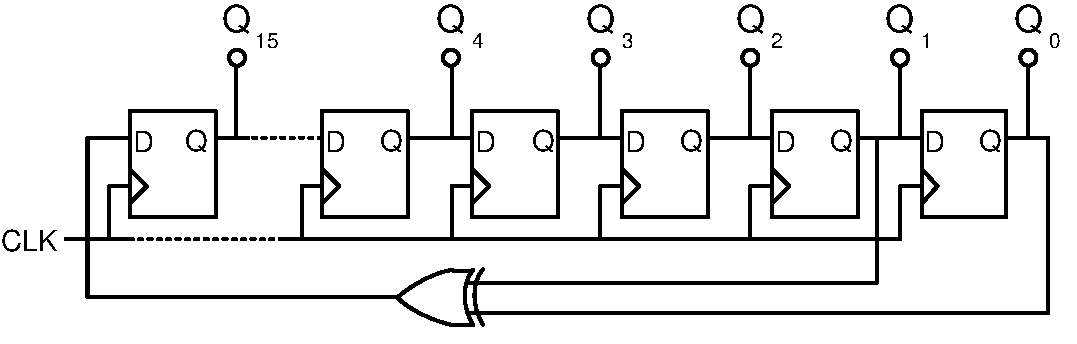
\includegraphics[width = 0.8\textwidth]{LFSR.pdf}
		\caption{16 Bit Linear Feedback Shift Register.}% \todo[inline]{Maybe change to IEEE symbols if we have time, AJR: we still have the eagle d-types but I think it would look a bit messy} }
   \label{fig:lfsr}
\end{figure}

A two input \texttt{XOR} gate is simulated using the \textbf{XOR} operation along with shifting to compare bits in different locations.
Bits $2$ and $4$ are used as inputs so a logical shift left by two is used to align them at the bit $4$ position. 
Masking the output value is used feedback to the top bit.
This is described using C in listing~\ref{lst:random.c}. 

\lstinputlisting[style=C,label=lst:random.c,caption=Linear Feedback Shift Register Subroutine]{pseudocode/random.c}





\subsection{Interrupt}
The code for the interrupt program is held in Appendix~\ref{sec:interrupt_appendix} listing~\ref{lst:interrupt.asm}.
This is the most complex example and makes use of both the multiply and factorial subroutines in sections~\ref{sec:multiply} and~\ref{sec:factorial} respectively.
The interrupt services the serial device by writing data to a $4$ byte circular buffer. 
A main program check to see if data is in the buffer then and if so calculates the factorial writing the result to the LEDs.
The buffer is purposefully small to test overflow.

\lstinputlisting[style=C,label=lst:interrupt.c,caption=Serial Device Interrupt Service Request]{pseudocode/interrupt.c}





%%  Simulation.tex
%  Document created by seblovett on hind.ecs.soton.ac.uk
%  Date created: Thu 27 Mar 2014 10:13:53 GMT
%  <+Last Edited: Sun 27 Apr 2014 15:41:59 BST by seblovett on seblovett-Ubuntu +>

\section{Simulation}

\subsection{Running the simulations}
\todo[inline]{A register window could also be done for this section too}

\todo[inline]{Sim.py needs a fair bit of change. If we have time, this could be altered to use Iains dir structure. This section highlights how to use his script and our assembler.}


How to run for each of the behavioural, extracted and mixed

Before the simulator is invoked, the assembler should be invoked. 
This is discussed in section~\ref{sect:runningassembler}. 
It can be done from within the programs directory (\texttt{~/design/fcde/verilog/programs}) by running, for example \texttt{assemble.py multiply}

The script ``simulate'' is an executable shell script. 
It is run from the terminal in the directory \texttt{~/design/fcde/verilog}. 
This supports running simulations of a full verilog model, cross simulation and a fully extracted simulation. 
Usage is as follows:\\
\begin{center}
\texttt{./simulate type program [definitions]}
\end{center}

The `type' can be one of the following: \textit{behavioural, mixed, extracted}.
`Program' is a relative path to the assembled hex file, usually located in the programs folder. 
Extra definitions can also be included to set the switch value or serial data input.

The serial data file used is located in the programs directory. 
This is a hex file with white space separated values of the form `` time data''. 
The data is then sent at the time to the processor by the serial module. 
An example serial data hex file is shown in listing~\ref{lst:serialdata}.

\lstinputlisting[label=lst:serialdata,caption={Example serial data file}]{../../Design/Implementation/programs/serial_data.hex}

Below is a complete list of commands to run all programs on all versions of the processor.
`Number' is a user defined decimal value to set the switches.
\begin{itemize}
\item \texttt{./assembler/assemble.py programs/multiply.asm \\ ./simulate behavioural programs/multiply.hex +define+switch\_value=number}
\item \texttt{./assembler/assemble.py programs/multiply.asm \\ ./simulate mixed programs/multiply.hex +define+switch\_value=number}
\item \texttt{./assembler/assemble.py programs/multiply.asm \\ ./simulate extracted programs/multiply.hex +define+switch\_value=number}\\

\item \texttt{./assembler/assemble.py programs/random.asm \\ ./simulate behavioural programs/random.hex +define+switch\_value=number}
\item \texttt{./assembler/assemble.py programs/random.asm \\ ./simulate mixed programs/random.hex +define+switch\_value=number}
\item \texttt{./assembler/assemble.py programs/random.asm \\ ./simulate extracted programs/random.hex +define+switch\_value=number}\\

\item \texttt{./assembler/assemble.py programs/factorial.asm \\ ./simulate behavioural programs/factorial.hex +define+switch\_value=number}
\item \texttt{./assembler/assemble.py programs/factorial.asm \\ ./simulate mixed programs/factorial.hex +define+switch\_value=number}
\item \texttt{./assembler/assemble.py programs/factorial.asm \\ ./simulate extracted programs/factorial.hex +define+switch\_value=number}\\

\item \texttt{./assembler/assemble.py programs/interrupt.asm \\ ./simulate behavioural programs/interrupt.hex programs/serial\_data.hex}
\item \texttt{./assembler/assemble.py programs/interrupt.asm \\ ./simulate mixed programs/interrupt.hex programs/serial\_data.hex}
\item \texttt{./assembler/assemble.py programs/interrupt.asm \\ ./simulate extracted programs/interrupt.hex programs/serial\_data.hex}
\end{itemize}

%\todo[inline]{how to run scan path sim too}

A scan path simulation can also be run.
This is done by running \texttt{ncverilog -sv +gui +ncaccess+r stimulus.sv  opcodes.svh cpu.sv} for a GUI or \texttt{ncverilog -sv stimulus.sv  opcodes.svh cpu.sv -exit} for a command line simulation.
This test pulses a signal on the SDI line, and verifies a pulse is seen on the output. 
The clock cycles, and therefore the number of registers, are counted and reported upon success of the simulation.

%\todo[inline]{need to mention extracting? i wouldn't say so as it should already be done and that can't really change.}

The number of clock cycles for each program to fully run is shown in table~\ref{tab:runtimes}. 
Factorial run time is given for an input of 8 and is the worst case. 
Interrupt is dependant on the serial data input and the time is given for the serial data file mentioned above.

\begin{table}
\centering
\caption{Clock cycles required for each program to run\todo[inline]{Make these more accurate when AJR has finished playing around}}
\label{tab:runtimes}
\begin{tabular}{|c|c|}
Program & Clock Cycles \\ \hline
Multiply	& 900	\\
Factorial	& 6000	\\
Random		& 	\\
Interrupt	& 30000	\\ \hline
\end{tabular}
\end{table}

%\todo[inline]{and TCL?}
A dissembler is also implemented in System Verilog to aid debugging.
It is an ASCII formatted array implemented at the top level of the simulation. 
It is capable of reading the instruction register with in the design, and reconstructing the assembly language of the instruction and is supported in behavioural, mixed and extracted simulations.
It will show the opcode, register addresses and immediate values.
It is automatically included by the TCL script.
The TCL script also opens a waveform window and adds important signals.


%\todo[inline]{check that the dissembler works in all the simulations (it doesn't\dots)}


%  Simulation.tex
%  Document created by seblovett on hind.ecs.soton.ac.uk
%  Date created: Thu 27 Mar 2014 10:13:53 GMT
%  <+Last Edited: Tue 29 Apr 2014 20:43:34 BST by seblovett on seblovett-Ubuntu +>

\section{Simulation}

\subsection{Running the simulations}
\todo[color=green,inline]{A register window could also be done for this section too}

%How to run for each of the behavioural, extracted and mixed

%What it does:

%Invokes assembler (if app) and simulation from anywhere. 
A python script, sim.py, was written to automatically invoke the assembler and simulator. 
The passed program is only assembled if the file exists with an extension of \texttt{.asm}. 
This allows for raw hex to be passed to the simulator where necessary. 
If a \texttt{.hex} file is passed, and a \texttt{.asm} file exists of the same name, the assembler will be invoked. 
The sim.py script is designed to be put on the user's path, allowing for the invocation of the assembler and simulator from anywhere. 

The usage for the script is:
\begin{center}
\texttt{sim.py [-t type] [-m module.sv / -p program.asm ] [ -s switchvalue ] [ -gdS ] [+define+extra\_definitions]}
\end{center}

%Supports all simualtions
All simulation types are supported. 
As well as full system simulations, the sim.py script also allows for other testbenches to be run.
All stimulus files are maintained in a directory and the testbenches can be run on verilog or magic modules. 
Where a Magic design is to be simulated, the script automatically extracts the netlist. 
This is done to prevent the Magic design and netlist being inconsistent. 
%Allows test benches to be run on both verilog and Magic modules. 

%Usage
The sim.py script provides a help prompt when run with \texttt{-h} or \texttt{--help} arguments. 
The help prompt is also displayed when incorrect arguments are supplied. 
The full help prompt is show in listing~\ref{lst:simpyhelp}. 

By default, the graphical user interface is not invoked. 
This can be done with the \texttt{-g} or \texttt{--gui} tags. 
A debug option, \texttt{-d}, exists when the user wants to get the majority of the simulation command, but modify it slightly. 

The program and module options should never be defined at the same time. 
One of them, however, should be. 
The program option is assembled, if necessary, and defined in the simulation command. 
The module option checks for the testbench file (identified by \textit{module}\_stim.sv) within the verification folder. 
The testbench is then used as the top level module. 

The type of simulation can be any of the folders in the verilog directory, for example \textit{behavioural}, \textit{mixed} or \textit{extracted}. 
A special type, \textit{magic} can be used.
When this is done so, the magic folder, \texttt{~/design/fcde/magic/design}, is checked for the module given. 
Type \textit{magic} and a program is equivalent to an extracted type simulation and is treated as such. 
The type is also given as a definition to the simulator, allowing reuse of test benches. 

The value of the switches can be easily defined by using the \texttt{-s} tag. 
The value given after this option is then passed to the simulator as a definition. 
If other definitions are required (for example, the serial data file), they can be defined, in full, in the trailing arguments. 
All trailing arguments are appended to the simulation command, allowing for the user to customise the invocation beyond the scope of the script. 

A scan path simulation can also be run.
This is done by running \texttt{./sim.py -S} and allows the same use described above for invoking the GUI.
If the \texttt{-S} option is defined, any program or module also given is ignored.
The scan path test pulses a signal on the SDI line, and verifies a pulse is seen on the output. 
The clock cycles, and therefore the number of registers, are counted and reported upon success of the simulation.


\lstinputlisting[label=lst:simpyhelp,caption={Help prompt for the sim.py script.}]{simpy.txt}



\subsection{Serial Data}

The serial data file used is located in the programs directory. 
This is a hex file with white space separated values of the form \textit{``time data''}.
Both values are given as hexadecimal numbers. 
The data is then sent at the time to the processor by the serial module. 
An example serial data hex file is shown in listing~\ref{lst:serialdata}.

\lstinputlisting[label=lst:serialdata,caption={Example serial data file}]{../../Design/Implementation/programs/serial_data.hex}


%\todo[inline]{how to run scan path sim too}


%\todo[inline]{need to mention extracting? i wouldn't say so as it should already be done and that can't really change.}

\subsection{Run Time}
The number of clock cycles for each program to fully run is shown in table~\ref{tab:runtimes}. 
Factorial run time is given for an input of 8 and is the worst case. 
Random is the time taken to compute a new value of the pseudo-random sequence. 
Interrupt is dependant on the serial data input and the time is given for the serial data file mentioned above.

\begin{table}
\centering
\caption{Clock cycles required for each program to run}%\todo[inline]{Make these more accurate when AJR has finished playing around}}
\label{tab:runtimes}
\begin{tabular}{|c|c|} \hline
Program & Clock Cycles \\ \hline
Multiply	& 1,100	\\
Factorial	& 5,700	\\
Random		& 2,500	\\
Interrupt	& 30,000	\\ \hline
\end{tabular}
\end{table}

%\todo[inline]{and TCL?}
\subsection{Simulation}

A dissembler is also implemented in System Verilog to aid debugging.
It is an ASCII formatted array implemented at the top level of the simulation. 
It is capable of reading the instruction register with in the design, and reconstructing the assembly language of the instruction and is supported in behavioural, mixed and extracted simulations.
It will show the opcode, register addresses and immediate values.
It is automatically included by the TCL script.
The TCL script also opens a waveform window and adds important signals.

\todo[color=green,inline]{Put a screen shot of the waveform window?}
%\todo[inline]{check that the dissembler works in all the simulations (it doesn't\dots)}


\newpage
\appendix
\definecolor{mygreen}{rgb}{0,0.6,0}
\lstset{ %
  backgroundcolor=\color{white},   % choose the background color; you must add \usepackage{color} or \usepackage{xcolor}
  basicstyle=\footnotesize,        % the size of the fonts that are used for the code
  breakatwhitespace=false,         % sets if automatic breaks should only happen at whitespace
  breaklines=true,                 % sets automatic line breaking
  captionpos=b,                    % sets the caption-position to bottom
  commentstyle=\color{mygreen},    % comment style
  deletekeywords={...},            % if you want to delete keywords from the given language
  escapeinside={\%*}{*)},          % if you want to add LaTeX within your code
  extendedchars=true,              % lets you use non-ASCII characters; for 8-bits encodings only, does not work with UTF-8
  frame=single,                    % adds a frame around the code
  keepspaces=true,                 % keeps spaces in text, useful for keeping indentation of code (possibly needs columns=flexible)
  keywordstyle=\color{black},       % keyword style
  language={[x86masm]Assembler},                 % the language of the code
  morekeywords={*,...},            % if you want to add more keywords to the set
  numbers=left,                    % where to put the line-numbers; possible values are (none, left, right)
  numbersep=5pt,                   % how far the line-numbers are from the code
  numberstyle=\tiny\color{black}, % the style that is used for the line-numbers
  rulecolor=\color{black},         % if not set, the frame-color may be changed on line-breaks within not-black text (e.g. comments (green here))
  showspaces=false,                % show spaces everywhere adding particular underscores; it overrides 'showstringspaces'
  showstringspaces=false,          % underline spaces within strings only
  showtabs=false,                  % show tabs within strings adding particular underscores
  stepnumber=2,                    % the step between two line-numbers. If it's 1, each line will be numbered
  stringstyle=\color{black},     % string literal style
  tabsize=4,                       % sets default tabsize to 2 spaces
  title=\lstname                   % show the filename of files included with \lstinputlisting; also try caption instead of title
}


\section{Code Listings}
All code listed in this section is passed to the assembler \emph{as is} and has been verfied using the final design of the processor.
\subsection{Multiply}
\label{sec:multiply}
\lstinputlisting[label=lst:multiply.asm,caption=multiply.asm]{../../Design/Implementation/programs/multiply.asm}
\subsection{Factorial}
\label{sec:factorial}
\lstinputlisting[label=lst:factorial.asm,caption=factorial.asm]{../../Design/Implementation/programs/factorial.asm}
\subsection{Random}
\label{sec:random}
\lstinputlisting[label=lst:random.asm,caption=random.asm]{../../Design/Implementation/programs/random.asm}
\subsection{Interrupt}
\label{sec:interrupt}
\lstinputlisting[label=lst:interrupt.asm,caption=interrupt.asm]{../../Design/Implementation/programs/interrupt.asm}


%  DeclarationofWork.tex
%  Document created by seblovett on seblovett-Ubuntu
%  Date created: Tue 29 Apr 2014 20:51:04 BST
%  <+Last Edited: Tue 29 Apr 2014 21:01:38 BST by seblovett on seblovett-Ubuntu +>

\section{Declaration of Work}

Table~\ref{tab:work} shows the break down of the work for this programming guide. 
Where multiple team members contributed to a section, approximate work percentages are given. 

\begin{table}
\caption{Work Breakdown for the Programmers Guide}
\label{tab:work}
\centering
\begin{tabular}{|c|c|} \hline
Chapter			&	User	\\ \hline
Introduction		&	hl13g10 \\	
Register Description	&	arr1g13 (50\%), hl13g10 (50\%) \\
Instruction Set		&	mw20g10	\\
Programming Tips	&	ajr2g10 (50\%), hl13g10 (50\%) \\		
Assembler		&	mw20g10 (75\%), hl13g10 (50\%) \\		
Programs		&	ajr2g10 \\
Simulation		&	hl13g10 \\
Code Listings		&	ajr2g10 \\ \hline
\end{tabular}
\end{table}


\end{document}

